\documentclass{article}
\usepackage{graphicx} % Required for inserting images
\setlength{\parskip}{\medskipamount}
\setlength{\parindent}{0pt}
\usepackage{natbib}

\title{Robustness of M}
\author{ernesto.jardim }
\date{October 2025}

\begin{document}

\maketitle

\section{Introduction}
\label{sec:introduction}

The accurate assessment of fish stock status is a foundational requirement for sustainable fisheries management worldwide. Quantitative stock assessment models, such as age-structured models, rely on several key demographic parameters to estimate population size, fishing pressure, and productivity. Among these, the rate of natural mortality ($M$), the loss of individuals due to causes other than fishing (e.g., predation, disease, starvation, senescence), is often the most critical and least understood component \cite{QuinnDeriso99, Haddon11}. When $M$ is estimated poorly or mis-specified, it can propagate substantial and misleading biases through the entire assessment, leading to inappropriate management advice, either resulting in stock depletion or unwarranted restrictions on fishing activity.

Despite its importance, natural mortality is rarely directly observable and must instead be estimated or assumed, often using empirical relationships based on life history traits such as maximum age, growth rate, or maturity \cite{Jensen96, Gislason10, then2014, kenchington2014}. This reliance on proxy relationships generates a pool of candidate $M$ models, each with different assumptions about the biological processes driving mortality (e.g., constant, age-dependent, or time-varying mortality) \cite{Liu22}. The choice of $M$ model therefore represents a major source of model uncertainty and mis-specification error in routine stock assessments. Given that the true underlying process of natural mortality is often unobservable or unknowable, analysts are faced with the challenge of selecting a working model that minimizes the potential for management failure.

The consequences of this mis-specification are high-stakes, translating directly into economic and ecological risk. According to \citep{Punt21} $M$ is positively correlated with biomass. As such, if the assessment model assumes an $M$ that is lower than the true rate, the stock's size and subsequent productivity will be underestimated, and vice-versa. When natural mortality is overestimated, the model assumes the stock is less productive and loses many individuals to natural causes. To reconcile this high loss with the observed catches, the model must estimate a significantly larger total biomass. Conversely, when M is underestimated, the model assumes the stock is more productive and resilient. Consequently, it estimates a smaller total biomass as being sufficient to explain the observed catches and abundance trends.

The challenge of model selection and parameter robustness is not unique to natural mortality, but is a pervasive issue in complex ecological and statistical models. Statistically, robustness is defined as the degree to which an estimator or model is resistant to departures from its underlying theoretical assumptions or from the true data generating process \cite{HilbornMangel97}. It acknowledges the fundamental reality that a model is a simplification or approximation of reality and hence will not reflect all of reality \cite{burnham2002}. In this framework, a robust parameter is one whose estimated value or resulting management advice remains stable and minimally biased even when the full, true underlying biological reality is not perfectly captured by the assessment model.

Our approach flips around the paradigm about $M$ model selection. Instead of trying to find the most realistic model, which is most of the times and impossible task due to the lack of observations, it focuses on selecting the "less worse" $M$ model, assessed by its resistance to mis-specifications in the context of providing policy advice. 

The central objective of this method is to give the analyst information about how to select a $M$ model that is most robust to mis-specifications of $M$ in the stock assessment. The methodology is based on a simulation-estimation framework to evaluate how poorly each candidate $M$ model performs when the estimation model assumes a different $M$ model than the operating model that represents the reference natural mortality model. By quantifying the magnitude and direction of bias induced by various forms of mis-specification, this analysis provides the stock assessment scientist with supporting information necessary to make the most risk-averse decision about the $M$ model to use, thereby enhancing the reliability and precautionary nature of the management advice.

\section{Methods}

To evaluate the robustness of the stock assessment model to mis-specification of natural mortality ($M$), we employed a simulation-testing approach within an Operating Model (OM) / Estimation Model (EM) framework. This method allows for the creation of a "ground truth" (the OM) from which pseudo-data are generated, and subsequently, the performance of the assessment model (the EM) can be tested when its assumptions regarding $M$ deviate from the OM's. 

The OMs were conditioned on a set of five distinct candidate models for natural mortality, based on their theoretical underpinnings and applicability to the biological characteristics of the study stock: the current model selected by the 2017? assessment benchmark (REF); the age based Chen-Watanabe model (REF), which incorporates growth parameters and maximum age; the constant Then et al. model (REF), based on the growth coefficient; the age based Lorenzen model (REF), which relates M to body weight; and the length based Brodziak et al model (REF), utilizing growth and reproductive parameters (Figure \ref{fig:mmodels}). These models represent distinct biological paradigms for mortality estimation and avoid redundancy that would over-weight particular model structures. We implemented a full factorial design (Table \ref{tab:design}) to systematically cross-test the impact of assuming one $M$ model when the underlying population dynamics are governed by another. This comprehensive design ensures that every candidate $M$ model serves as both a potential "true" state in an OM and a potential "mis-specified" assumption in an EM. The factorial design consisted of 20 unique combinations where each of the five models served as the conditioning model for an OM, which was then assessed using each of the four alternative models as mis-specified M inputs. This yielded four mis-specification scenarios per OM. The diagonal elements of the design matrix, where conditioning and estimation $M$ models matched, were used as baseline reference cases for evaluating bias.

\begin{figure}[h!]
	\centering
	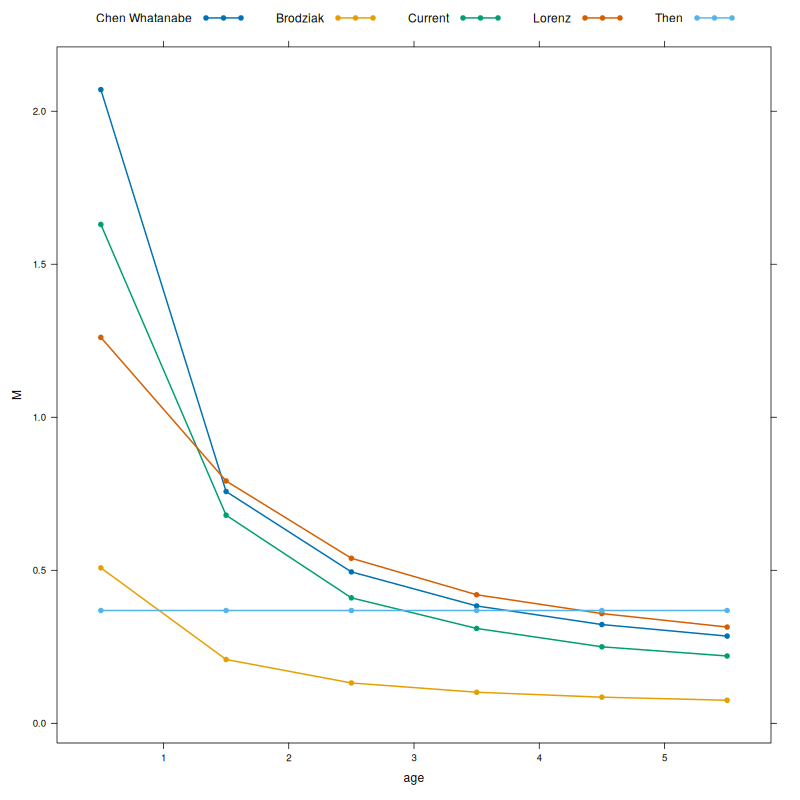
\includegraphics[width=0.75\linewidth]{mmodels}
	\caption{$M$ models used in this analysis}
	\label{fig:mmodels}
\end{figure}


\begin{table}
	\begin{tabular}{c||ccccc}
		\hline
		 & & & EM & & \\
		OM & Current & Chen Watanabe & Then & Lorenz & Brodziak \\
		\hline
		\hline
		Current & * & x & x & x & x \\
		Chen Watanabe & x & * & x & x & x \\
		 Then & x & x & * & x & x \\
		Lorenz & x & x & x & * & x \\
		Brodziak & x & x & x & x & * \\
		\hline
	\end{tabular}
	\caption{Natural mortality models robustness analysis simulation design. "x" refers to scenarios used to evaluate robustness of $M$ model to mis-specification. "*" refers to scenarios used to check bias. "OM" = Operating Model, "EM" = Estimation Model}
	\label{tab:design}
\end{table}

From each of the four conditioned OMs, we generated multiple stochastic realizations of pseudo-observations. These simulated datasets were designed to mimic the data typically available for this stock, specifically fisheries-dependent catch-at-age matrices and one or more fisheries-independent indices of abundance. For each OM 250 iterations were generated to ensure that observation error, a key component of uncertainty in real-world assessments, was adequately propagated through the analysis. These simulated datasets formed the complete set of inputs for the subsequent estimation (EM) phase of the experiment.

The core of the robustness test involved executing the full factorial design by systematically mis-specifying the $M$ vector within the EM. For each set of simulated data generated from a specific OM (e.g., data from OM-Lorenz), we fitted the stock assessment model four separate times. In each of these four fits, the $M$ matrix used by the EM was replaced with one generated by one of the candidate models (i.e., EM-Lorenz, EM-ChenWatanabe, EM-Then, EM-Brodziak). This process directly creates the scenarios of interest: cases on the diagonal of the design matrix (Table \ref{tab:design}) where $M_{OM} = M_{EM}$ serve as a control, while the 20 off-diagonal cases represent the impact of $M$ mis-specification.

Finally, we quantified the impact of $M$ mis-specification by comparing the outputs of the EM fits against the known values from the OM used to generate the data. The primary performance metric was the Root Mean Square Error (RMSE) computed over the time series of fishing mortality ($F$), which provides a standardized measure of both the bias and precision of $F$ estimates resulting from an incorrect $M$ assumption. Additional performance statistics, such as the relative error in terminal Spawning Stock Biomass (SSB) and recruitment ($R$), were also computed to provide a more holistic understanding of the consequences of mis-specification on key stock status indicators and management advice. All simulations and analyses were conducted using the \texttt{FLR} libraries and the \texttt{a4a} (assessment for all) framework within the R statistical environment.

\section{Results}

\subsection{Sensitivity to changes in von bertalanffy parameters}

Brodziak e Then models very sensitive to von bertalanffy parameter k and the former also to minimum length.

\begin{figure}[h!]
	\centering
	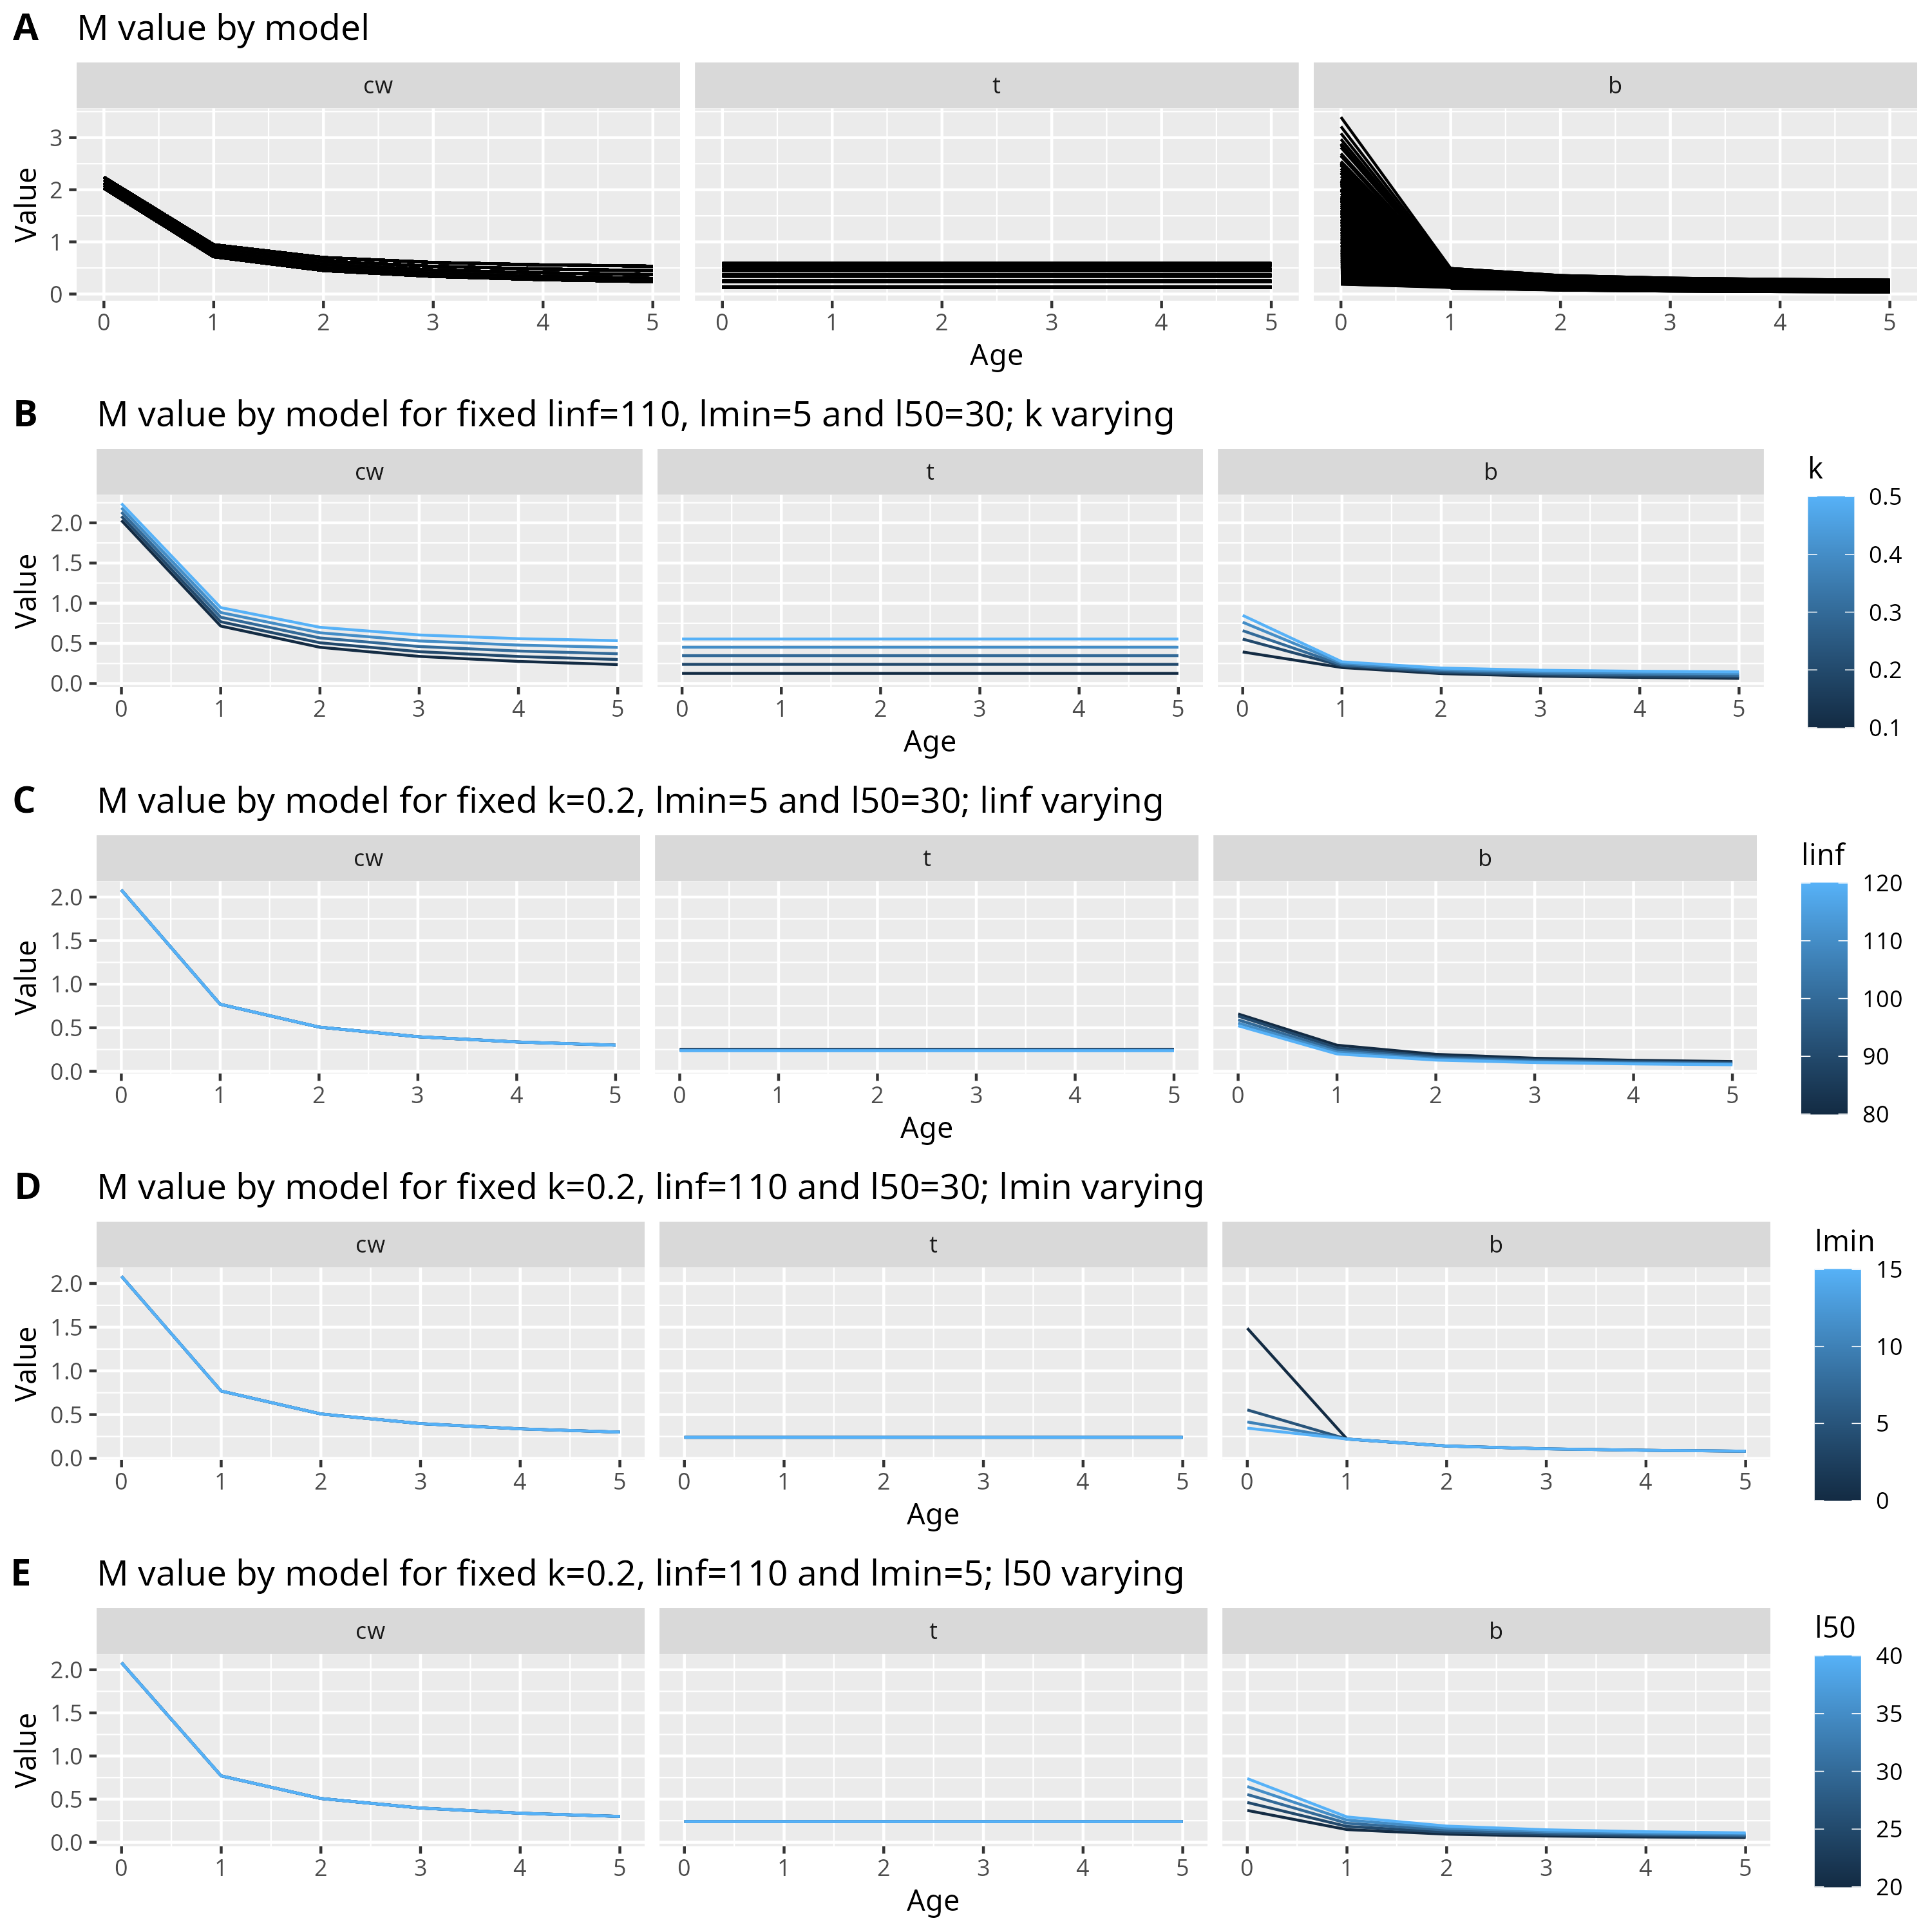
\includegraphics[width=0.95\linewidth]{sensitivity_plot.png}
	\caption{Analysis of the impact of von bertalanffy parameters in $M$ by age models Chen Watanabe, Lorenz, and Then}
	\label{fig:vbsensitivity}
\end{figure}

\subsection{Assessing estimator bias}

To assess the potential bias introduced by the estimator model, we proceed with comparing the results obtain by the estimator when the $M$ model matched the operating model's. The model will be fitted to each OM iteration and should be able to estimate population abundance, fishing mortality and catch at age without bias.

This analysis will give confidence that the outcome of the estimator when the $M$ model is mis-specified reflect the impact of the mis-specification and not a bias introduced by the estimator model.  


\subsection{Robustness to mis-specification of the model}

Constant models are a weird option, considering they're widely used although are probably the worst natural mortality representation one can find. It's unrealistic to consider natural mortality to be the same across all ages.



\bibliographystyle{plain}
\bibliography{biblio}

\end{document}
